% !TEX TS-program = pdflatex
% !TEX encoding = UTF-8 Unicode

% This is a simple template for a LaTeX document using the "article" class.
% See "book", "report", "letter" for other types of document.

\documentclass[11pt]{article} % use larger type; default would be 10pt
\usepackage{polski}
\usepackage{mathtools}
\usepackage{amssymb}
\usepackage{hyperref}
\usepackage{adjustbox,lipsum}

\usepackage[utf8]{inputenc} % set input encoding (not needed with XeLaTeX)

%%% Examples of Article customizations
% These packages are optional, depending whether you want the features they provide.
% See the LaTeX Companion or other references for full information.

%%% PAGE DIMENSIONS
\usepackage{geometry} % to change the page dimensions
\geometry{a4paper} % or letterpaper (US) or a5paper or....
% \geometry{margin=2in} % for example, change the margins to 2 inches all round
% \geometry{landscape} % set up the page for landscape
%   read geometry.pdf for detailed page layout information

\usepackage{graphicx} % support the \includegraphics command and options

% \usepackage[parfill]{parskip} % Activate to begin paragraphs with an empty line rather than an indent

%%% PACKAGES
\usepackage{booktabs} % for much better looking tables
\usepackage{array} % for better arrays (eg matrices) in maths
\usepackage{paralist} % very flexible & customisable lists (eg. enumerate/itemize, etc.)
\usepackage{verbatim} % adds environment for commenting out blocks of text & for better verbatim
\usepackage{subfig} % make it possible to include more than one captioned figure/table in a single float
% These packages are all incorporated in the memoir class to one degree or another...

%%% HEADERS & FOOTERS
\usepackage{fancyhdr} % This should be set AFTER setting up the page geometry
\pagestyle{fancy} % options: empty , plain , fancy
\renewcommand{\headrulewidth}{0pt} % customise the layout...
\lhead{}\chead{}\rhead{}
\lfoot{}\cfoot{\thepage}\rfoot{}

%%% SECTION TITLE APPEARANCE
\usepackage{sectsty}
\allsectionsfont{\sffamily\mdseries\upshape} % (See the fntguide.pdf for font help)
% (This matches ConTeXt defaults)

%%% ToC (table of contents) APPEARANCE
\usepackage[nottoc,notlof,notlot]{tocbibind} % Put the bibliography in the ToC
\usepackage[titles,subfigure]{tocloft} % Alter the style of the Table of Contents
\renewcommand{\cftsecfont}{\rmfamily\mdseries\upshape}
\renewcommand{\cftsecpagefont}{\rmfamily\mdseries\upshape} % No bold!

%%% END Article customizations

%%% The "real" document content comes below...

\title{Metody odkrywania wiedzy: Forest Cover Type Prediction}
\author{Monika Pawluczuk, Bartosz Lemiec}
%\date{} % Activate to display a given date or no date (if empty),
         % otherwise the current date is printed 

\begin{document}
\maketitle

\section{Interpretacja tematu projektu}

Temat dotyczy predykcji typu lasu i oparty jest na danych dostarczonych przez US Forest Service (USFS). 

Celem jest przewidzenie zalesienia terenu, a dokładniej określeniu typu drzewa dominującego w danym terenie, z danych kartograficznych. Typ zalesienia został określony, na parcelach o powierzchni 30x30 metrów, przez US Forest Service (USFS). Dane są nieprzeskalowane i zawierają kolumny z wartościami binarnymi dla niezależnych zmiennych jakościowych takich jak obszar czy też typ gleby.

\section{Opis algorytmów wykorzystanych w badaniach}
\subsection{Algorytm K-najbliższych sąsiadów}

Algorytm może być stosowany zarówno do zadań klasyfikacji jak i regresji. Jest jednym z najbardziej znanych podejść aproksymacji funkcji na podstawie zapamiętywania. W celu wyznaczenia odpowiedzi na zapytanie dotyczące przykładu bierze się pod uwagę najbliższy mu, według przyjętej metryki, przykład trenujący.  

Tak sformułowany algorytm nie wymaga żadnych założeń co do dziedziny i reprezentacji przykładów, oprócz określenie miary odległości. Funkcja miary będzie w rzeczywistości pojęciem, o przeciwdziedzinie będącej zbiorem kategorii.

Algorytm charakteryzuje się bardzo dużą szybkością uczenia się, a jego dokładność zależy od ilości przykładów trenujących oraz funkcji mierzącej odległość.

Zostanie wykorzystany pakiet R class (\url{https://cran.r-project.org/web/packages/class/class.pdf}). Zakłada on użycie jako metryki odległości euklidesowej.

\subsection{Drzewo decyzyjne - algorytm C4.5}

Algorytm wykorzystywany do generowania drzew decyzyjnych. Jest rozszerzeniem wcześniejszego algorytmu ID3. Drzewa decyzyjne generowane za pomocą tego algorytmu mogą zostać wykorzystane przy klasyfikacji i dlatego też algorytm ten określany jest często jako klasyfikator statystyczny.

Buduje on drzewo decyzyjne z zestawu danych trenujących, wykorzystując pojęcie entropii informacji. Zestaw trenujący zawiera zaklasyfikowane już przykłady, zawierające p-wymiarowy wektor $\ (x_{1,i}, x_{2,i}, …, x_{p,i}) $, gdzie $\ x_j $ reprezentuje wartość atrybutu albo właściwości próbki, oraz klasę do której $\ S_i $ należy.

Przy każdym węźle drzewa decyzyjnego, algorytm C4.5, wybiera atrybut danych, który z największą efektywnością rozdziela zbiór próbek na podzbiory o większej entropii dla którejś z klas. Kryterium podziału jest entropia względna. Atrybut o największym przyroście informacji jest wybierany, jako ten  na podstawie którego tworzone będą kolejne węzły lub liście. Algorytm C4.5 następnie postępuje rekurencyjnie, aby stworzyć pomniejsze podlisty.

Algorytm z góry pokrywa kilka podstawowych przypadków:

\begin{itemize}
\item Wszystkie próbki w liście należą do tej samej klasy $\ \Rightarrow $ w takim przypadku drzewo tworzy liść drzewa wybierający daną klasę.
\item Żaden z atrybutów nie niesie ze sobą jakichkolwiek informacji $\ \Rightarrow $ algorytm C4.5 wykorzystuje węzeł decydujący wyżej w strukturze drzewa i wartość oczekiwaną w nim zawartą.
\item Instancja nigdy nie spotkanej wcześniej klasy zostaje znaleziona $\ \Rightarrow $ algorytm tworzy węzeł wyżej w drzewie wykorzystując jego wartość oczekiwaną.
\end{itemize}

Zostanie wykorzystany pakiet R RWeka, zawierający implementację algorytmu J48
(\url{https://cran.r-project.org/web/packages/RWeka/RWeka.pdf}).

\subsection{Naiwny klasyfikator bayesowski}

Naiwny klasyfikator bayesowski reprezentuje hipotezy za pomocą oszacowań (tworzonych na podstawie zbioru trenującego) pewnych prawdopodobieństw i klasyfikuje przykłady, wybierając dla nich najbardziej prawdopodobne kategorie. Przypomina on optymalny klasyfikator bayesowski, z podstawową różnicą, że nie wykorzystuje żadnych innych hipotez (nawet w celach pomocniczych). Zakłada on ograniczenie się do zestawu atrybutów dyskretnych.

Na podstawie zbioru trenującego szacowane są prawdopodobieństwa poszczególnych kategorii pojęcia docelowego c oraz prawdopodobieństwa poszczególnych wartości atrybutów dla przykładów różnych kategorii. Będą nas interesować oszacowania prawdopodobieństw:

\begin{itemize}
\item Prawdopodobieństwo dla każdej możliwej kategorii pojęcia docelowego \emph{c} 
\item Prawdopodobieństwo wystąpienia danej wartości atrybutu dla przykładu z danej klasy - dla każdej możliwej kategorii pojęcia docelowego i każdej wartości każdego atrybutu.
\end{itemize}

Aby obliczyć prawdopodobieństwo kategorii \emph{d} pojęcia docelowego: wyznaczamy ile jest przykładów z tą klasą w zbiorze trenującym, a następnie dzielimy ją przez ilość wszystkich przykładów w zbiorze trenującym.

Podobnie, aby oszacować prawdopodobieństwo wartości atrybutu $\ a_i=v $ dla kategorii \emph{d}, liczymy ile jest przykładów każdej kategorii dla poszczególnych wartości każdego atrybutu i dzielimy uzyskaną przez liczbę wszystkich przykładów tej kategorii.

Wadą tego podejścia jest przypadek, gdy w którejś z grup nie ma żadnego przykładu. Wówczas prawdopodobieństwo jest szacowane na 0, co jest bardzo radykalnym podejściem. W związku z tym stosuje się technikę wygładzania, która jest też zaimplementowana w pakiecie, który będzie użyty w projekcie. 

Wygładzanie polega na zastąpieniu wartości zerowej pewną niewielką, lecz dodatnią wartością $\ \epsilon $. Jest to proste i popularne rozwiązanie, które powinno być dostosowane do do rozmiaru zbioru trenującego. Na pewno wartość ta powinna być mniejsza niż odwrotność liczebności tego zbioru (skoro grupa, której mamy tylko jeden przykład będzie miała prawdopodobieństwo $\ 1/|T| $  - grupa o zerowej liczbie przykładów powinna mieć mniejsze prawdopodobieństwo).

Najczęstszą heurystyką jest przyjęcie epsilonu na poziomie połowy odwrotności liczebności zbioru trenującego $\ 1/2*|T| $.

Ta sama zasada obowiązuje również przy obliczaniu prawdopodobieństwa klas.

Zostanie wykorzystany pakiet R e1071 (\url{https://cran.r-project.org/web/packages/e1071/e1071.pdf}). Implementacja zakłada niezależność rozkładów atrybutów (stąd “naiwność” w nazwie) i rozkład Gaussa. Niestety implementacja, w razie brakujących wartości atrybutów pomija przykład ze zbioru trenującego.

\section{Plan badań}

\subsection{Cel badań}

Obszar przeznaczony do analizy zawiera cztery lokalizacje w Roosevelt National Forest, znajdującego się w północnym Colorado. Każda obserwacja przeprowadzona została na obszarze 30x30m. Celem jest predykcja typu lasu, który pokrywać będzie dany obszar, w postaci liczby, która to z kolei odpowiada jednemu z siedmiu typów:

\begin{center}
    \begin{tabular}{ | l | l | }
    \hline
    	Lp. & Nazwa \\ \hline
    	1 &Świerk/jodła \\
	2 & Sosna wydmowa \\
	3 & Sosna żółta \\
	4 & Topola/wierzba \\
	5 & Topola osikowa \\
	6 & Daglezja zielona \\
	7 & Drzewo karłowate \\ \hline
    \end{tabular}
\end{center}

\subsection{Charakterystyka zbiorów danych i ich przygotowanie}

Zestaw trenujący złożony z 15120 przykładów zawiera zarówno właściwości, jak i typ pokrycia. Zestaw testowy zawiera jedynie właściwości. Celem jest przewidzenie typu pokrycia w każdym z wierszy zestawu testowego (565892 obserwacje).

\subsubsection{Kolumny danych}

\noindent\adjustbox{max width=\textwidth}{

    \begin{tabular}{ | l | l | l | l |}
    \hline
    	Lp. & Nazwa & Opis & Opis (j.ang.)\\ \hline
    	1 & Elevation & Elewacja wyrażona w metrach & Elevation in meters \\
    	2 & Aspect & Strona wyrażona w stopniach azymutu & Aspect in degrees azimuth \\
    	3 & Slope  & Nachylenie wyrażone w stopniach & Slope in degrees \\
	4 & Horizontal\_Distance\_To\_Hydrology & Dystans horyzontalny do najblizszego zbiornika wodnego & Horizontal distance to nearest surface water features \\
	5 & Vertical\_Distance\_To\_Hydrology & Dystans wertykalny do najblizszego zbiornika wodnego & Vertical distance to nearest surface water features \\
6 & Horizontal\_Distance\_To\_Roadways & Dystans horyzontalny do najbliższej drogi & Horizontal distance to nearest roadway \\
7 &Hillshade\_9am & Cieniowanie, zakres od 0 do 255, o godzinie 9, w dniu przesilenia & Hillshade index at 9am, summer solstice (0 to 255 index) \\
8 & Hillshade\_Noon & Cieniowanie, zakres od 0 do 255, w południe, w dniu przesilenia & Hillshade index at noon, summer solstice (0 to 255 index) \\
9 
& Hillshade\_3pm & Cieniowanie, zakres od 0 do 255, o godzinie 3, w dniu przesilenia & Hillshade index at 3pm, summer solstice (0 to 255 index) \\
10 & Horizontal\_Distance\_To\_Fire\_Points & Dystans horyzontalny do najbliższej stacji straży pożarnej & Horz Dist to nearest wildfire ignition points \\
11 & Wilderness\_Area & Obszar, wyrażony binarnie, w 4 kolumnach & Wilderness area designation \\
12 & Soil\_Type & Rodzaj gleby, wyrażony binarnie, w 40 kolumnach & Soil Type designation (40 binary columns, 0 = absence or 1 = presence) \\
13 & Cover\_Type & Docelowy typ zalesienia, wartości od 1 do 7 & Forest Cover Type designation (7 types, integers 1 to 7) \\ \hline
    	\end{tabular}
}

\subsubsection{Typy obszarów}

\begin{center}
    \begin{tabular}{ | l | l | }
    \hline
    	Lp. & Nazwa \\ \hline
    	1 &Rawah Wilderness Area \\
	2 & Neota Wilderness Area \\
	3 & Comanche Peak Wilderness Area \\
	4 & Cache la Poudre Wilderness Area \\ \hline
    \end{tabular}
\end{center}

\subsubsection{Rodzaje gleb}

\noindent\adjustbox{max width=\textwidth}{

    \begin{tabular}{ | l | l | l |}
    \hline
Lp.
& Nazwa
& Opis \\ \hline
1
& Cathedral family
& Rock outcrop complex, extremely stony \\
2
& Vanet
& Ratake families complex, very stony \\
3
& Haploborolis
& Rock outcrop complex, rubbly \\
4
& Ratake family
& Rock outcrop complex, rubbly \\
5
& Vanet family
& Rock outcrop complex complex, rubbly \\
6
& Vanet - Wetmore families
& Rock outcrop complex, stony \\
7
& Gothic family
& - \\
8
& Supervisor
& Limber families complex \\
9
& Troutville family
& Very stony \\
10
& Bullwark - Catamount families - Rock outcrop complex, rubbly
& - \\
11
& Bullwark - Catamount families - Rock land complex, rubbly
& -  \\
12
& Legault family
& Rock land complex, stony \\
13
& Catamount family
& Rock land - Bullwark family complex, rubbly \\
14
& Pachic Argiborolis
& Aquolis complex \\
15
& unspecified in the USFS Soil and ELU Survey
& - \\
16
& Cryaquolis
& Cryoborolis complex \\
17
& Gateview family
& Cryaquolis complex \\
18
& Rogert family, very stony
& - \\
19
& Typic Cryaquolis
& Borohemists complex \\
20
& Typic Cryaquepts
& Typic Cryaquolls complex \\
21
& Typic Cryaquolls
& Leighcan family, till substratum complex \\
22
& Leighcan family, till substratum, extremely bouldery
& - \\
23
& Leighcan family, till substratum - Typic Cryaquolls complex
& - \\
24
& Leighcan family, extremely stony
& - \\
25
& Leighcan family, warm, extremely stony
& - \\
26
& Granile
& Catamount families complex, very stony \\
27
& Leighcan family, warm
& Rock outcrop complex, extremely stony \\
28
& Leighcan family
& Rock outcrop complex, extremely stony \\
29
& Como
& Legault families complex, extremely stony \\
30
& Como family - Rock land
& Legault family complex, extremely stony \\
31
& Leighcan
& Catamount families complex, extremely stony \\
32
& Catamount family - Rock outcrop
& Leighcan family complex, extremely stony \\
33
& Leighcan - Catamount families
& Rock outcrop complex, extremely stony \\
34
& Cryorthents
& Rock land complex, extremely stony \\
35
& Cryumbrepts - Rock outcrop
& Cryaquepts complex \\
36
& Bross family - Rock land
& Cryumbrepts complex, extremely stony \\
37
& Rock outcrop - Cryumbrepts
& Cryorthents complex, extremely stony \\
38
& Leighcan - Moran families
& Cryaquolls complex, extremely stony \\
39
& Moran family - Cryorthents
& Leighcan family complex, extremely stony \\
40
& Moran family - Cryorthents
& Rock land complex, extremely stony \\ \hline
    \end{tabular}
}

\section{Wstępna analiza danych}
Wstępna analiza danych została przedstawiona w tabeli poniżej, gdzie zostały policzone podstawowe wartości, takie jak ilość unikalnych wartości atrybutu, wartość minimalna, maksymalna, czy mediana.

\subsection{Podsumowanie dostępnych danych}

Liczba przykładów trenujących: 15120
Liczba kolumn:  56
Rozkład obszarów zalesienia:

\begin{center}
    \begin{tabular}{ llllllll }
    \hline
    	Typ lasu & 1 & 2 & 3 & 4 & 5 & 6 & 7 \\ \hline
    	Ilość przykładów & 2160 & 2160 & 2160 & 2160 &  2160 & 2160 & 2160 \\ \hline
    \end{tabular}
    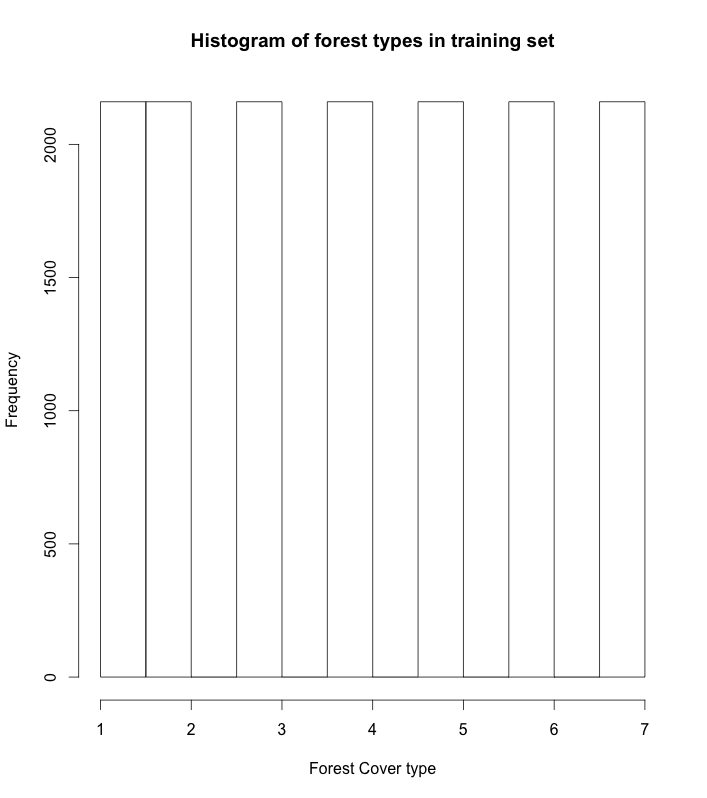
\includegraphics[width=8cm, height=8cm]{histogram}
\end{center}

\begin{itemize}
\item Zbiór trenujący zawiera 15120 wierszy, wraz z 56 kolumnami
\item Kolumna 1 reprezentuje ID danego wpisu
\item Kolumny 2-11 reprezentują atrybuty ilościowe
\item Kolumny 12-15 to reprezentacja binarna obszaru \emph{Wilderness\_Area} (4 kolumny wzajemnie się wykluczające: ComachePeak, CachePodure, Neota, Rawah)
\item Kolumny 16-55 to reprezentacja binarna typu gleby \emph{Soil\_Type} (40 kolumn wzajemnie się wykluczających)
\item Kolumna \emph{Cover\_Type} zawiera 7 wartości (docelowa klasyfikacja)
\item Kolumny binarne wzajemnie się wykluczają
\end{itemize}

Największą zależność, pod względem przypisania do klasy docelowej, wykazuje atrybut \emph{Elevation}, który to został przedstawiony na poniższym wykresie pudełkowym:

\begin{center}
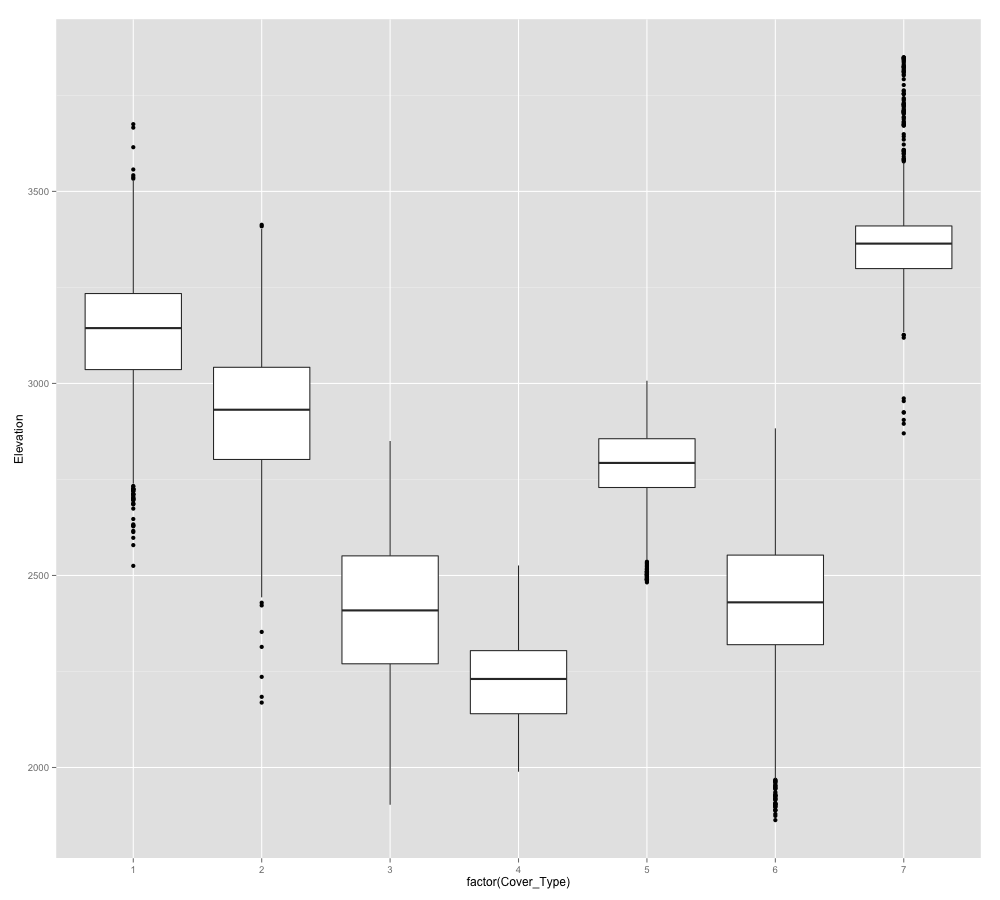
\includegraphics[width=8cm, height=8cm]{boxplot}
\end{center}

Można więc się spodziewać, że na przykład w przypadku zastosowania algorytmu C4.5 będzie on stanowił atrybut wyjściowy, od którego algorytm będzie zaczynać budowanie drzewa, a dopiero analiza kolejnych wartości atrybutów pozwoli na dokładniejsze zaklasyfikowanie próbki.

\subsection{Atrybut dyskretny reprezentujący pojęcie docelowe}

Atrybutem reprezentującym pojęcie docelowe jest typ lasu. Jest to zbiór liczbowy, składający się z siedmiu wartości:

\begin{center}
    \begin{tabular}{ | l | l | l | }
    \hline
    	Lp. & Nazwa & Nazwa (j.ang.) \\ \hline
    	1 &Świerk/jodła & Spruce/Fir \\
	2 & Sosna wydmowa & Lodgepole Pine \\
	3 & Sosna żółta & Ponderosa Pine \\
	4 & Topola/wierzba & Cottonwood/Willow \\
	5 & Topola osikowa & Aspen \\
	6 & Daglezja zielona & Douglas-fir \\
	7 & Drzewo karłowate & Krummholz \\ \hline
    \end{tabular}
\end{center}

\subsection{Przetworzenie do odpowiedniej postaci}

Zbiór danych trenujących jest dostępny do pobrania w postaci pliku csv. Jest on wczytywany za pomocą komendy read.csv do formatu data.frame.

Algorytm najbliższych sąsiadów jako argument danych treningowych/testujących może przyjmować dane w tym właśnie formacie, podobnie jak naiwny klasyfikator bayesowski i algorytm C4.5.

\subsubsection{Modyfikacja atrybutów}

Ze względu na wzajemne wykluczanie się wartości przechowywanych w kolumnach 12-15, opisujących \emph{Wilderness\_Area}, atrybut ten został złączony w jeden, przyjmujący wartości dyskretne od 1 do 4, gdzie jego liczba porządkowa przypisana jest do typu obszaru opisanego w tabeli Typy obszarów.

Podobna optymalizacja została przeprowadzona dla typów gleb \emph{Soil\_Type} (kolumny 16-55), z tego samego powodu. Przyjmują one więc wartości dyskretne od 1 do 40 zgodnie z tabelą Rodzaje gleb.

\subsubsection{Eliminacja/naprawa defektów danych}

Dane nie zawierają brakujących danych, dlatego też nie będzie potrzebna estymacja wartości atrybutów dla danych brakujących. Ewentualne defekty w danych mogą występować ze względu na źródło danych, skąd zostały one pobrane (USFS), jednak przy realizacji tego projektu zakładamy ich poprawność, ze względu na trudność lokalizacji ewentualnych błędów.

\subsubsection{Modyfikacja rozkładu klas}

Klasy w zestawie danych testowych rozkładają się równomiernie, dlatego też nie zostanie przeprowadzona modyfikacja ich rozkładu.

\subsubsection{Losowanie podzbiorów danych}

Ze względu na równy podział klas, losowanie podzbiorów danych wykonywane będzie z uwzględnieniem sprawiedliwego podziału rozkładu klas pomiędzy zbiorami danych trenujących. Oznacza to, iż każdy podzbiór danych zbioru trenującego będzie zawierać równą ilość klas konkretnego typu tak, aby w modelu uczącym się żadna z klas nie mogła zdominować pod względem jej wyboru.

\subsubsection{Możliwość zdefiniowania nowych atrybutów}

Możliwość definicji nowych atrybutów może wyniknąć z korelacji zachodzących pomiędzy istniejącymi atrybutami. Korelacja zaobserwowana będzie w trakcie dalszej części realizacji projektu, na podstawie graficznej reprezentacji atrybutów.

\subsubsection{Ustalenie kryteriów lub algorytmu selekcji atrybutów}

\textbf{Parametry algorytmów wymagające dostrojenia}

\emph{Naiwny klasyfikator Bayesowski}
\begin{itemize}
\item ustalenie wartości \emph{threshold}, którą będą zastępowane prawdopodobieństwa równe zeru bądź mniejsze od $\ \epsilon $
\item ustalenie granicy prawdopodobieństwa - $\ \epsilon $, która będzie zastępowana wartością threshold
\end{itemize}

\emph{Algorytm k-najbliższych sąsiadów}
\begin{itemize}
\item ustalenie wartości \emph{k} - ilu najbliższych sąsiadów ma być branych pod uwagę
\item ustalenie wartości \emph{l} - minimalna ilość głosów potrzebna do podjęcia ostatecznej decyzji
\end{itemize}

\subsubsection{Miary jakości i ocena modelu}

Ocena modelu polega na ocenie według dwóch kategorii:
\begin{enumerate}
\item Trafność klasyfikacji (Classification / Predictive accuracy)
	\begin{enumerate}
	\item Miary True Positive Rate, True Negative Rate
	\item Macierz pomyłek
	\item Analiza krzywej ROC
	\item Feature importance
	\end{enumerate}
\item Szybkość i skalowalność
	\begin{enumerate}
	\item czas uczenia się
	\item szybkość klasyfikowania
	\end{enumerate}
\end{enumerate}

\section{Implementacja i wyniki}

\subsection{Stworzone modele}

\subsubsection{Algorytm C.45}

Algorytm C4.5 został zaimplementowany jako funkcja \emph{J48}  w pakiecie RWeka.

Tworzenie samego modelu drzewa decyzyjnego zostało przetestowane dla różnych opcji:
\begin{itemize}
\item wszystkie opcje klasyfikatora z domyślnymi wartościami

\begin{center}
    \begin{tabular}{ | l | l | l | }
    \hline
    	Correctly Classified Instances & 9311 & 61.5807 \% \\ \hline
	Incorrectly Classified Instances & 5809 & 38.4193 \% \\ \hline
    \end{tabular}
\end{center}

\item (Weka control: Do not collapse tree, O = TRUE)

\begin{center}
    \begin{tabular}{ | l | l | l | }
    \hline
    	Correctly Classified Instances & 9311 & 61.5807 \% \\ \hline
	Incorrectly Classified Instances & 5809 & 38.4193 \% \\ \hline
    \end{tabular}
\end{center}

\item tworzenie jedynie binarnych podziałów (Weka control: Use binary splits only, B = TRUE)

\begin{center}
    \begin{tabular}{ | l | l | l | }
    \hline
    	Correctly Classified Instances & 12529 & 82.8638 \% \\ \hline
	Incorrectly Classified Instances & 2591 & 17.1362 \% \\ \hline
    \end{tabular}
\end{center}

\item nieprzycinanie drzew (Weka control: Use unpruned tree, U = TRUE)

\begin{center}
    \begin{tabular}{ | l | l | l | }
    \hline
    	Correctly Classified Instances & 13809 & 91.3294 \% \\ \hline
	Incorrectly Classified Instances & 1311 & 8.6706 \% \\ \hline
    \end{tabular}
\end{center}

\end{itemize}

Spośród przetestowanych modeli wybrano najlepszy. Model ten został następnie przetestowane za pomocą metody cross-validation: dzielono zestaw danych treningowych na \emph{k} podzbiorów o równej liczności, a następnie uczono model na jednym z tych zbiorów i testowano na \emph{(k-1)} pozostałych. Przetestowano tą metodę dla każdego $\ k \in \{1, ..., |training\_data|\} $. Sprawdzono w ten sposób stabilność algorytmu.

Wydawałoby się, że najlepsze wyniki zostały uzyskane przy zablokowaniu przycinania drzew - daje ono największy odsetek dobrze sklasyfikowanych przykładów. Istnieje jednak niebezpieczeństwo, że jest to kwestia nadmiernego dopasowania drzewa do danych treningowych. Za pomocą metody cross-validation widać, że obawy potwierdzają się - przy dzieleniu danych na mniejsze zbiory, jakość klasyfikatora natychmiast spada. Poniżej przedstawiono wykres zależności stopnia poprawnie sklasyfikowanych przykładów od ilości zbiorów na które podzielono zbiór treningowy.

\begin{center}
	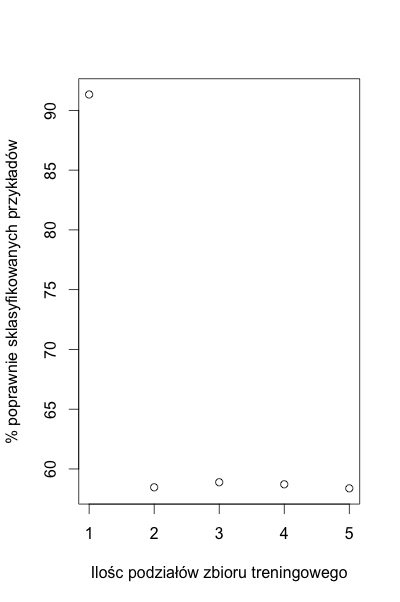
\includegraphics[height=8cm]{unprunned-overfitting}
\end{center}

W związku z tym, za najlepszą metodę uznano uzyskiwanie drzewa jedynie przy podziałach binarnych. Kolejnym etapem jest maksymalne przycięcie drzewa, które jednocześnie nie powodowałoby dużej straty jakości modelu. Jest to ustalane za pomocą opcji \emph{M}, które ustala minimalną liczbę przykładów, dla których może być utworzony liść - domyślnie jest to liczba 2. Niestety powiększanie tej wartości ma mocny wpływ na jakość modelu, co można zobaczyć na wykresie poniżej.

\begin{center}
	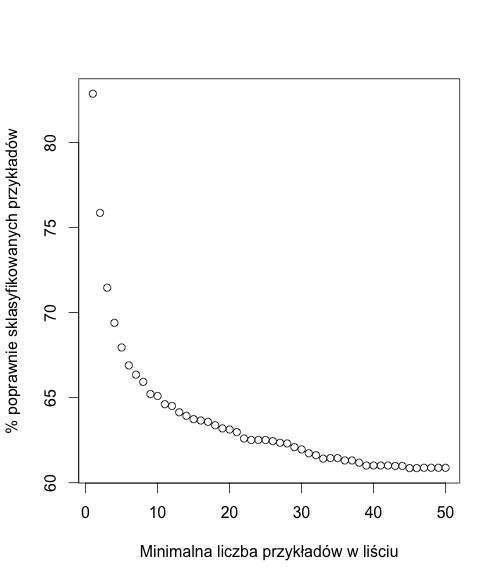
\includegraphics[height=8cm]{binaryTree-minimumLeaf}
\end{center}

W związku z tym domyślna wartość pozostanie aby nie stracić poziomu minimalizacji. Ostatnim etapem jest upewnienie się, że stworzony model jest odporny i zachowuje swoją skuteczność przy trenowaniu na podzielonych zbiorach danych.

\subsubsection{Naiwny klasyfikator Bayesowski}


\subsubsection{Algorytm k-najbliższych sąsiadów}

Algorytm k-najbliższych sąsiadów został zaimplementowany jako funkcja \emph{IBk}  w pakiecie RWeka.

Tworzenie samego modelu klasyfikacji zostało przetestowane dla różnych opcji:
\begin{itemize}
\item wszystkie opcje klasyfikatora z domyślnymi wartościami

\begin{center}
    \begin{tabular}{ | l | l | l | }
    \hline
    	Correctly Classified Instances & 15120 & 100 \% \\ \hline
	Incorrectly Classified Instances & 0 & 0 \% \\ \hline
    \end{tabular}
\end{center}

Model jest jednak zbytnio dopasowany, dlatego przy sprawdzaniu modelu metodą cross-validation, jego jakość drastycznie spada:

\begin{center}
	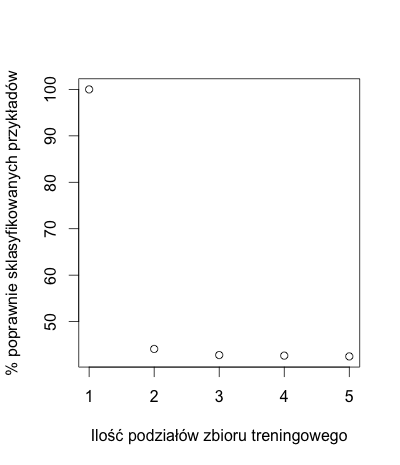
\includegraphics[height=8cm]{knn-cross-validation}
\end{center}

Przy zwiększaniu liczby branych pod uwagę sąsiadów, jakość klasyfikatora również spada:

\begin{center}
	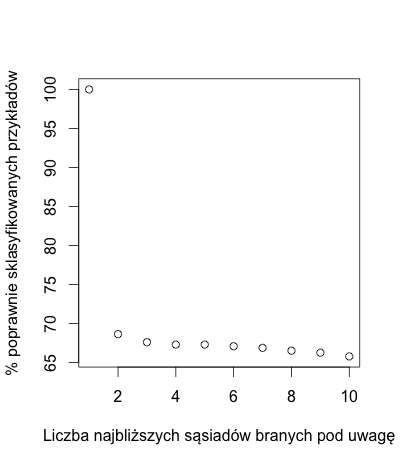
\includegraphics[height=8cm]{knn-neighbours}
\end{center}

\end{itemize}

\subsection{Ocena stworzonych modeli}

\subsubsection{Algorytm C4.5}

\subsubsection{Naiwny klasyfikator Bayesowski}

\subsubsection{Algorytm k-najbliższych sąsiadów}

\end{document}
